\documentclass[11pt]{article}
\usepackage[a4paper, portrait, margin=1in]{geometry}
\usepackage{graphicx}
\usepackage{listings}


\begin{document}

\title{Advanced Systems Lab (Fall'15) -- First
Milestone}

\author{Name: \emph{Sandro Huber}\\Legi number: \emph{10-924-777}}

\date{
\vspace{4cm}
\textbf{Grading} \\
\begin{tabular}{|c|c|}
\hline  \textbf{Section} & \textbf{Points} \\ 
\hline  1.1 &  \\ 
\hline  1.2 &  \\ 
\hline  1.3 &  \\ 
\hline  2.1 &  \\ 
\hline  2.2 &  \\ 
\hline  2.3 &  \\ 
\hline  3.1 &  \\ 
\hline  3.2 &  \\ 
\hline  3.3 &  \\ 
\hline  3.4 &  \\ 
\hline  3.5 &  \\ 
\hline  3.6 &  \\ 
\hline \hline Total & \\
\hline 
\end{tabular} 
}

\maketitle

\newpage

\section{System Description}\label{sec:system-description}

\subsection{Database}\label{sec:database}

Length: 1-2 pages

Start by explaining the schema of the database and the indexes used to
speed up data access. Describe the interface to the database (queries
and stored procedures).

Make sure to explain the design in terms of what you wanted to achieve,
what decisions you took and what is the expected behavior.

Include baseline performance characteristics of the database (max
throughput, response time, and scalability).

\subsubsection{Schema and Indexes}\label{sec:schema-and-indexes}
\begin{figure}[!ht]
\centering
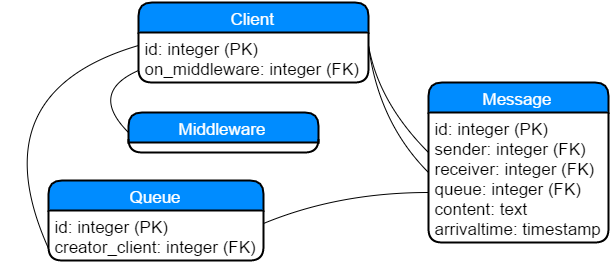
\includegraphics[width=0.7\linewidth]{figures/database/db_schema}
\caption{The Database Schema}
\label{fig:db_schema}
\end{figure}
The database schema was chosen in such a way, that it provides all required functionality, but is still easy to setup and maintain. The following lines shortly illuminate the tables and their column types.
\begin{itemize}
	\item \textbf{Client}: Guarantees through the serial datatype that each client in the whole system has a unique ID and stores which client is registered on which middleware. This can be handy when wanting an even distribution of clients over all middlewares.
	\item \textbf{Queue}: Stores all queues created by clients. Also ensures that all queues are unique.
	\item \textbf{Middleware}: A sequence which is used to get a unique ID for each middleware joining the system.
	\item \textbf{Message}: Here, all messages sent by clients are stored. The foreign keys ensure that we only get messages from valid clients registered in the system. As one can see, the content column is of type text, despite the choice of varchar(200) or varchar(2000) may be more obvious with respect to the system requirements. Find my thoughts about this choice in section \ref{sec:design-decisions}.
\end{itemize}
To speed up the data access I used the two following indices:
\begin{lstlisting}[language=SQL,basicstyle=\small]
(a) INDEX msg_rcvr_q_idx ON MESSAGE (RECEIVER, QUEUE);
(b) CREATE INDEX msg_sndr_idx ON MESSAGE (SENDER);
\end{lstlisting}
The reasoning behind the choice of them is based on the following thoughts. The indices in a database system affect search time, i.e. filtering of rows with respect to a criterion. Since the whole system is built with predefined stored procedures (find a full list in section \ref{sec:stored-procedures}) we know exactly what these filter parameters will be. To simplify the view, only the most relevant parts of the queries are shown (query they belong to in brackets):
\begin{lstlisting}[language=SQL,basicstyle=\small,escapeinside={(*@}{@*)}]
(1) WHERE RECEIVER (*@(get\_queues\_for\_client)@*)
(2) WHERE RECEIVER AND QUEUE (*@(read\_all\_messages\_of\_queue)@*)
(3) WHERE RECEIVER AND QUEUE ORDER BY ARRIVALTIME (*@(remove\_top\_message\_from\_queue)@*)
(4) WHERE RECEIVER AND SENDER ORDER BY ARRIVALTIME (*@(read\_message\_from\_sender)@*)
\end{lstlisting}
Since an index on two columns (c1, c2) is also an index onto c1, we can see that the index (a) already covers the WHERE clauses of (1)-(3). In addition with index (b) we get a full coverage of all queries having to filter some data. It is intentional that there is no index on the GROUP BY of ARRIVALTIME. Find more about the reasoning in section \ref{sec:design-decisions}.

\subsubsection{Stored Procedures}\label{sec:stored-procedures}
Every database access is done via a stored procedure. This allows to have a single point of failure, maintenance and control over functionality. Having this lone entry guarantees fast and reliable feature implementation and debugging. In Java the stored procedures are interfaced via Prepared Statments, which can be cached by the VM, such that only the dynamic parameter values have to get fetched, before a query can be executed. The following stored procedures are implemented:
\begin{lstlisting}
create_queue(creator_client INTEGER)
delete_queue(queue_id INTEGER)
register_client(on_middleware INTEGER)
get_queues_for_client(client_receiver INTEGER)
read_all_messages_of_queue(receiver_id INTEGER, queue_id INTEGER)
read_message_from_sender(sender_id INTEGER, receiver_id INTEGER)
remove_top_message_from_queue(receiver_id INTEGER, queue_id INTEGER)
send_message(sender_id INTEGER,
	receiver_id INTEGER, queue_id INTEGER, content TEXT)
register_middleware()
get_registered_clients()
get_number_of_messages()
get_registered_queues()
take_stamp()
\end{lstlisting}

\subsubsection{Design decisions}\label{sec:design-decisions}
The design aims to be simple, but yet complex enough to provide all necessary functionalities through a nice interface. Please find in the following lines the reasoning about some design decision I took while implementing the system:
\begin{itemize}
	\item \textbf{text vs varchar(n)}: First of all, all datatypes char(n), varchar(n), varchar and text are internally all converted to the same C data structure varlena. So from the performance perspective no (major) differences are measurable. Because I wanted to be flexible and send messages of length 200 and 2000 in the same setup I decided to go with the flexible variant text. Choosing varchar(2000) for every case is bad, because the unused space when inserting smaller strings will be filled with spaces and thus not give any performance advantages.
	\item \textbf{Ghost-Client}: Since messages can also be addressed to all clients in the system, I introduced a ghost-client with an ID of 0, which gets created right at the database initialization. This ghost-client allows that instead of having RECEIVER=NULL, we have RECEIVER=0 for all broadcast messages, which is internally much easier to handle.
	\item \textbf{Index on ARRIVALTIME}: Maintaining an index is not cheap for a database system, so it's wise to use them with caution. Because of that I decided that the indices (1) and (2) are already discarding enough rows, such that the sorting operation is not too costly anymore.
	\item \textbf{ARRIVALTIME location}: The ARRIVALTIME is implemented as a trigger on the database. Another, also valid choice, would have been to let the client set it. But because I wanted to minimize the work of the clients and guarantee a unique timestamp on each message I did choose the trigger-option.
\end{itemize}
receiver = 0
content = text and not varchar
no index on group by of arrivaltime
1 main table -> no update, only simple insert/delete queries
trigger/arrivaltime on db and not on client side
\subsubsection{Performance characteristics}\label{sec:performance-characteristics}

\subsection{Middleware}\label{sec:middleware}

Length: 1-2 pages

Explain the design from a high-level point of view, highlighting what
you wanted to achieve, design decisions, expected behavior.

Then go into more detail on how the middleware connects to the database
and clients, and how queuing is implemented.

Show what are the performance characteristics of the middleware
(i.e.~throughput, latency, scalability).

\subsubsection{Design overview}\label{sec:design-overview}

\subsubsection{Interfacing with clients}\label{sec:interfacing-with-clients}

\subsubsection{Queuing and Connection pool to database}\label{sec:queuing-and-connection-pool-to-database}

\subsubsection{Performance characteristics}\label{sec:performance-characteristics-1}

\subsection{Clients}\label{sec:clients}

Length: 2-3 pages

Explain the interface of the clients to your messaging system and their
high level design, including the ways you have instrumented the code for
debugging and benchmarking purposes.

Provide a detailed description of the workloads used later in the report
(operation mix, starting and ending state of the database, assumptions
on workload behavior). Explain how the load was generated (include
baselines on load generation speed) and how the clients were deployed.

Which are the sanity checks in place for ensuring correct load
generation and validity of responses?

\subsubsection{Design and interface}\label{sec:design-and-interface}

\subsubsection{Instrumentation}\label{sec:instrumentation}

\subsubsection{Workloads and deployment}\label{sec:workloads-and-deployment}

\subsubsection{Sanity checks}\label{sec:sanity-checks}

\section{Experimental Setup}\label{sec:experimental-setup}

Length: 1-2 pages

Explain the overall design of the complete system and list the
configurations (number of middlewares, number of clients, types of
machines, communication patterns) corresponding to the main workloads.

Describe the mechanisms for deploying the system for experiments and the
way performance numbers are gathered and processed. Make the description
so that someone unfamiliar with your system can replicate the steps, and
reference the different script files you submit as code in the SVN
repository.

\subsection{System Configurations}\label{sec:system-configurations}

\subsection{Configuration and Deployment mechanisms}\label{sec:configuration-and-deployment-mechanisms}

\subsection{Logging and Benchmarking mechanisms}\label{sec:logging-and-benchmarking-mechanisms}

\section{Evaluation}\label{sec:evaluation}

Length: up to 10 pages

In this section we expect to see the different experiments you ran to
exercise the system, and with each experiment we expect a clear
description of the system configuration used, the hypothesis on behavior
and the explanation of the behavior observed (in terms of the different
design decisions taken beforehand) -- \emph{missing either of these for
an experiment might make you lose all points for that given experiment!}
Keep in mind that for a good explanation of the results of an experiment
you might have to use one or more methods of data analysis presented in
the lecture and in the book.

See below for a short description on what each part should contain.

\subsection{System Stability}\label{sec:system-stability}

To prove that your system functions correctly and that it is stable
include the trace of a 30 minute run, plotting both response time and
throughput. Use at least 30 clients (sending and receiving data), 2
middlewares and a non-empty database.

\subsection{System Throughput}\label{sec:system-throughput}

Measure the maximum throughput of the system (describe the exact
configuration and workload, and the reasoning behind choosing these
particular ones) and show the average response time for this experiment.

\subsection{System Scalability}\label{sec:system-scalability}

Explain the different configurations used to explore the scalability of
your system, and the outcomes of these experiments in terms of
throughput and response times. The main goal of this subsection is to
define the ranges in which your system operates best.

\subsection{Response Time Variations}\label{sec:response-time-variations}

Report and analyze how the response times change in the system with
different message sizes, different number of clients and different
number of middleware nodes.

\subsection{$2^k$ Experiment}\label{sec:k-experiment}

Conduct a 2\^{}k analysis of your system (aim at exploring non-obvious
interactions of parameters). Use the methods learned in this lecture to
conduct the detailed analysis.

\subsection{Conclusion}\label{sec:conclusion}

To conclude the report summarize the behavior of the system in terms of
the design and the representative workloads. Finally, outline in a few
points what would you do differently if you could design the system
anew.

\end{document}
